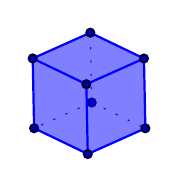
\begin{tikzpicture}%
	[x={(0.681462cm, -0.327528cm)},
	y={(0.731633cm, 0.326817cm)},
	z={(-0.017949cm, 0.886519cm)},
	scale=1.000000,
	back/.style={loosely dotted, thin},
	edge/.style={color=blue, thick},
	facet/.style={fill=blue,fill opacity=0.500000},
	vertex/.style={inner sep=1pt,circle,draw=blue!25!black,fill=blue!75!black,thick,anchor=base}]
%
%
%% Coordinate of the vertices:
%%
\coordinate (-0.50000, -0.50000, 0.50000) at (-0.50000, -0.50000, 0.50000);
\coordinate (-0.50000, 0.50000, -0.50000) at (-0.50000, 0.50000, -0.50000);
\coordinate (-0.50000, 0.50000, 0.50000) at (-0.50000, 0.50000, 0.50000);
\coordinate (0.50000, 0.50000, -0.50000) at (0.50000, 0.50000, -0.50000);
\coordinate (0.50000, -0.50000, -0.50000) at (0.50000, -0.50000, -0.50000);
\coordinate (0.50000, 0.50000, 0.50000) at (0.50000, 0.50000, 0.50000);
\coordinate (0.50000, -0.50000, 0.50000) at (0.50000, -0.50000, 0.50000);
\coordinate (-0.50000, -0.50000, -0.50000) at (-0.50000, -0.50000, -0.50000);
%%
%%
%% Drawing edges in the back
%%
\draw[edge,back] (-0.50000, 0.50000, -0.50000) -- (-0.50000, 0.50000, 0.50000);
\draw[edge,back] (-0.50000, 0.50000, -0.50000) -- (0.50000, 0.50000, -0.50000);
\draw[edge,back] (-0.50000, 0.50000, -0.50000) -- (-0.50000, -0.50000, -0.50000);
%%
%%
%% Drawing vertices in the back
%%
\node[vertex] at (-0.50000, 0.50000, -0.50000)     {};
%%
%%
%% Drawing the facets
%%
\fill[facet] (0.50000, -0.50000, 0.50000) -- (0.50000, -0.50000, -0.50000) -- (0.50000, 0.50000, -0.50000) -- (0.50000, 0.50000, 0.50000) -- cycle {};
\fill[facet] (0.50000, -0.50000, -0.50000) -- (-0.50000, -0.50000, -0.50000) -- (-0.50000, -0.50000, 0.50000) -- (0.50000, -0.50000, 0.50000) -- cycle {};
\fill[facet] (0.50000, -0.50000, 0.50000) -- (-0.50000, -0.50000, 0.50000) -- (-0.50000, 0.50000, 0.50000) -- (0.50000, 0.50000, 0.50000) -- cycle {};
%%
%%
%% Drawing edges in the front
%%
\draw[edge] (-0.50000, -0.50000, 0.50000) -- (-0.50000, 0.50000, 0.50000);
\draw[edge] (-0.50000, -0.50000, 0.50000) -- (0.50000, -0.50000, 0.50000);
\draw[edge] (-0.50000, -0.50000, 0.50000) -- (-0.50000, -0.50000, -0.50000);
\draw[edge] (-0.50000, 0.50000, 0.50000) -- (0.50000, 0.50000, 0.50000);
\draw[edge] (0.50000, 0.50000, -0.50000) -- (0.50000, -0.50000, -0.50000);
\draw[edge] (0.50000, 0.50000, -0.50000) -- (0.50000, 0.50000, 0.50000);
\draw[edge] (0.50000, -0.50000, -0.50000) -- (0.50000, -0.50000, 0.50000);
\draw[edge] (0.50000, -0.50000, -0.50000) -- (-0.50000, -0.50000, -0.50000);
\draw[edge] (0.50000, 0.50000, 0.50000) -- (0.50000, -0.50000, 0.50000);
%%
%%
%% Drawing the vertices in the front
%%
\node[vertex] at (-0.50000, -0.50000, 0.50000)     {};
\node[vertex] at (-0.50000, 0.50000, 0.50000)     {};
\node[vertex] at (0.50000, 0.50000, -0.50000)     {};
\node[vertex] at (0.50000, -0.50000, -0.50000)     {};
\node[vertex] at (0.50000, 0.50000, 0.50000)     {};
\node[vertex] at (0.50000, -0.50000, 0.50000)     {};
\node[vertex] at (-0.50000, -0.50000, -0.50000)     {};
%%
%%
\end{tikzpicture}